\documentclass{article}
\usepackage[a4paper,landscape]{geometry}
\usepackage{pdfpages}
\usepackage{tikz}
\usepackage{hyperref}
\usepackage{fancyhdr}

\begin{document}
\pagenumbering{gobble}

\title{Unveil}
\author{Filip Dobrocky}
\newcommand{\theyear}{2025}
\newcommand{\version}{v1.0}
\newcommand{\instruments}{a (string) instrument and live electronics}

\makeatletter

\fancyhf{}
\renewcommand{\headrulewidth}{0pt}
\fancyfoot[c]{}
\fancypagestyle{FirstPage}{
  \lfoot{
    \small
    \copyright\theyear\ \@author
    \hspace{\stretch{1}}
    \href{https://filip-dobrocky.github.io}{filip-dobrocky.github.io}
    \hspace{\stretch{1}}
    filip.dobrocky@gmail.com
  }
}

\renewcommand{\maketitle}{
  \begin{center}
    \vspace*{\fill}
    {\Huge\bfseries \@title \par}
    \vskip 0.5em
    {\large for \instruments}
    \vskip 2em
    {\Large \@author}
    \vskip 1em
    {\large \version}
    \vspace*{\fill}
  \end{center}
}
\makeatother

\maketitle
\thispagestyle{FirstPage}

\newpage

\section*{Introduction}
The intention of the piece is to create a gradually unfolding immersive soundscape created exclusively from live input of a string instrument.
The focus is put on the texture and timbral transitions, from pitch to noise and vice versa.
Certain parts are live-looped (including the effects and transitions, see \nameref{system_structure}) and repeated later in the composition to create layered spatial textures.
These loops are also used for spectral freezing controlled by the live input.

The score itself is supposed to serve as an outline for the composition, with various degrees of freedom, so that each interpretation is different, and only the general structure is fixed.
It is indicated where various parameters of the system should be changed, but the indications are not strict and can be interpreted freely.

The score has 5 movements where different techniques and approaches are used.
The movements should come after one another in a more or less continuous flow, without longer pauses.
The total approximate duration is \textbf{13 minutes}, but is not strict.

The notation is based on time durations indicated by horizontal dashed lines. The approximate times are marked at barlines, where each bar is 20 seconds long.
Non-pitched sounds are notated by cross noteheads, while pitched sounds are notated by regular noteheads.
The pitches are not absolute and only approximate. Various bowed string instrument techniques are indicated,
although with slight modifications, the score can be adapted also for non-string instruments,
which are capable of producing sustained pitched and non-pitched sounds and preferably can be captured by contact microphones.

The whole live electronics system is implemented as a SuperCollider script, although several extensions are required: \href{https://github.com/ambisonictoolkit/atk-sc3}{The Ambisonic Toolkit (ATK)}, \href{https://github.com/JamesWenlock/AmbiVerbSC}{AmbiVerbSC} and \href{https://github.com/supercollider/sc3-plugins}{sc3-plugins}.

The piece, including the SC files and the score, is available at this \href{https://github.com/filip-dobrocky/unveil-live-electronics}{GIT repository}.

\newpage
\section*{System structure} \label{system_structure}

\begin{center}
\begin{minipage}{0.62\textwidth}
\usetikzlibrary {graphs, graphdrawing}
\usegdlibrary{layered}
\tikz
  \graph [layered layout, branch right=2.5cm] {
      { "mic inputs" [edges={line width=1.5pt}],
        "loop 1",
        "loop 2",  
        "loop 3"
      }
      -> "resonator"
      -> [edges={line width=1.5pt}]
         "pitch shifter"
      -> [edges={line width=1.5pt}]
         "destroyer"
      -> [edges={line width=1.5pt}]
         "reverb"
      -> { "loop 1", "loop 2", "loop 3" }
      -> spatialization
      -> [edges={line width=1.5pt}]
         "ambisonic reverb"
      -> [edges={line width=1.5pt}]
         "speaker system";

      "mic inputs" -> "spectral freeze"
      -> "resonator";

      "loop 1" -> "spectral freeze";
      "loop 2" -> "spectral freeze";
      "loop 3" -> "spectral freeze";
      "reverb" -> "spatialization";
  };
\end{minipage}%
\hfill
\begin{minipage}{0.34\textwidth}
\textbf{System Notes}

This system uses multiple independed loops with variable length (dependend on the first recording), the input of which is post-FX. 
There are several effects: \textit{resonator, pitch shifter, destroyer} (bit crushing and downsampling), and a tank \textit{reverb} based on the Dattorro algorithm.

Moreover, there is a \textit{spectral freeze} effect which freezes the spectrum of the current position in given loops dependend on the live input amplitude.
The individual frozen spectra can be crossfaded with the input signal.

With the default configuration, there are 5 signals to which effects are applied individually: 2 microphone inputs and 3 loops (altough these numbers can be changed and this setup can be modified for particular purposes).

These signals are spatialized: 
evenly panned in a circle using ambisonic encoding. 
The sound field then can be shaped using ambisonic techniques \textit{Push} 
(pushes the sound field into a plane wave coming from given direction), 
\textit{Rotate} (rotation along the X axis) and \textit{Tumble} (rotation along the Z axis).
FOA is used in this version.
There is also an ambisonic tank reverb at the end of the chain (\texttt{AmbiVerbSC}).
The ambisonic signals can be decoded to various speaker setups and also to binaural output for headphone monitoring.

Further details about the system can be found in the SuperCollider script \texttt{unveil.scd}.

\end{minipage}
\end{center}

\newpage
\section*{Controller mapping}
This is a MIDI mapping currently used in the script for Novation Launchcontrol XL.
It can be adapted for other controllers by modifying given environment variables in the SuperCollider script. 
\begin{figure}[h]
\centering
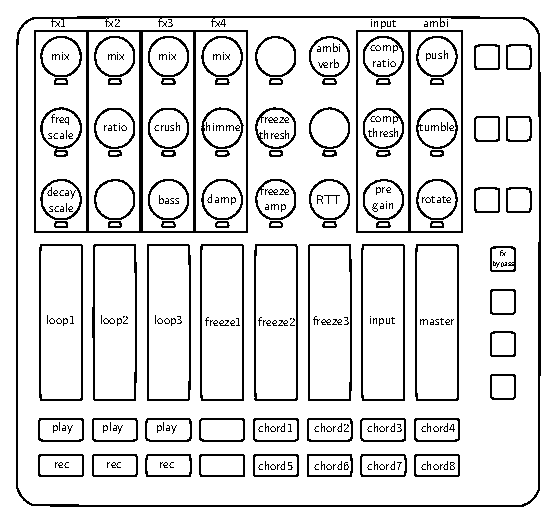
\includegraphics[width=0.55\textwidth]{ctl_mapping.eps}
\end{figure}

\newpage

\includepdf[pages=-]{./ly/score.pdf}  % Include all pages from your score

\end{document}